\section{Kacper Poznański}
\centering\title{\textbf{Pierwsza zasada termodynamiki}}
\\
\textbf{Definicja Pierwszej zasady dynamiki:} Energię wewnętrzną możemy zmienić przez wykonanie nad ciałem pracy lub przekazanie ciepła.
\\
Wzór \textbf{Pierwszej zasady termodynamiki} często formułuje się jako: 

\centering \(ΔEw = W + Q\).

\begin{itemize}
    \item ΔEw - zmiana energi wewnętrznej ciała
    \item W - praca wykonana przez otoczenie ciała lub ciało
    \item Q - ciepło dostarczone do ciała
\end{itemize}

Zmiana energii wewnętrznej ciała ΔEw jest równa sumie pracy W wykonanej nad tym ciałem oraz dostarczonego mu ciepła Q, Tak jak pokazane na obrazie\ref{fig1}
\begin{figure}[htbp]
    \centering
    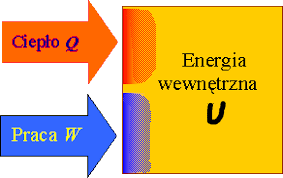
\includegraphics[]{pictures/ciepl.png}
    \caption{Obraz4}
    \label{fig1}
\end{figure}
\begin{table}[!h]
\begin{tabular}{ll}
\hline
\begin{tabular}{|ll|}
\hline
\multicolumn{1}{|l|}{Przykład}         & Energia wewnętrzna zmieniła się w wyniku:  \\ \hline
\multicolumn{1}{|l|}{Pocierając ręką o rękę czujemy ciepło}                    &
wykonania pracy  \\ \hline
\multicolumn{1}{|l|}{Stojąc obok kominka czujemy ciepło} & przepływu ciepła \\ \hline
\end{tabular}  
\end{tabular}
\end{table}
\textbf{Wnioskami Pierwszej Zasady Termodynamiki są:}

\begin{enumerate}
    \item W układzie zamkniętym energia nie ginie i nie powstaje, może tylko zmieniać się z jednej postaci w drugą.
    \item Praca i ciepło są równoważnymi sposobami przekazywania energii i są wyrażane w tych samych jednostkach \textit{1J dżul}.
    \item Energia układu zamkniętego, który nie wymienia ciepła i nie wykonuje pracy (ani nie jest nad nim wykonywana praca) nie zmienia się.
    \item \underline{nie jest możliwe} zbudowanie układu który by tworzył ciepło nie pobierając go z otoczenia \textit{tzw. perpetum mobile}.
\end{enumerate}




